\documentclass[main.tex]{subfiles}
\ProvidesPackage{preamble}

\usepackage[nottoc]{tocbibind}
\usepackage[english]{babel}
\usepackage[utf8]{inputenc}
\usepackage[table]{xcolor}
\usepackage[nohead, nomarginpar, margin=1in, foot=.25in]{geometry}
\usepackage{tabularx}
\usepackage{graphicx}
\usepackage{float}
\usepackage[english]{babel}
\usepackage{paralist}
\usepackage{datetime}
\usepackage{afterpage}

\begin{document}

\section{Design}

\subsection{General Design Decisions}
We have chosen pandas dataframes \cite{pandas} as the common data format for both data exchange and any calculations. Pandas provides us with data structures ``that cohere with the rest of the scientific Python stack`` \cite{mckinney2011pandas}, such as NumPy, which we are using to calculate historical returns and risk metrics (\ref{BL Structure}). Additionally, it is supported natively by many third party APIs and can even be used to read data from SQL databases. For additional information, please consult the official pandas documentation \cite{pandas}.

\subsection{Overview of System Architecture}

Before discussing any specific component and architectural layer in depth, it is worth revisiting our original architecture \cite{TR}.
\begin{figure}[H]
    \caption{Original Thalia System Architecture \cite{TR}}
	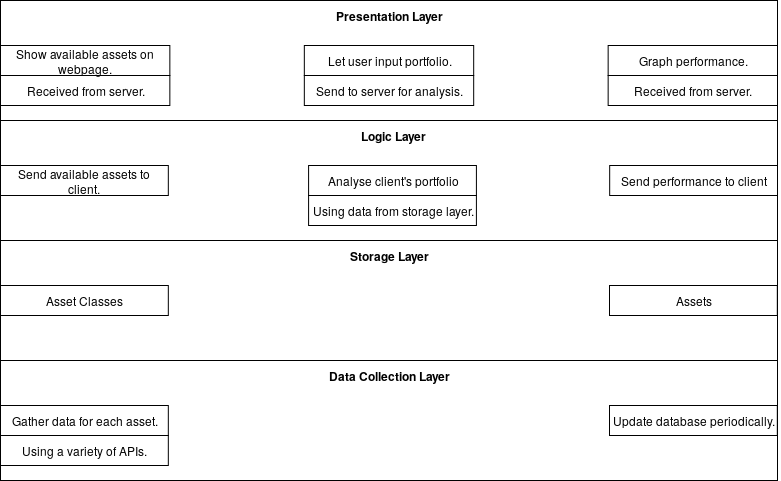
\includegraphics[width=\textwidth]{04Design/04Pictures/architecture_layer_diagram.png}
\end{figure}
The above schematic illustrates how we modified a typical Three Layer architecture [citation needed] to include a Data Collection Layer. Subsequent discussion will refer to this layer as the `Data Harvester`. It consists of adapters for third party APIs which offer price data for financial assets. The associated API will be queried according to a configurable interval to allow for live updates to our price data. Additionally, initial seeding of the database with historical price data can also be achieved via the Data Harvester. The decision to isolate this system component has been made in order to increase security by limiting the acess of the Thalia web service to the financial data database to read-only and to allow for independent scaling of the Data Harvester and our web service \cite{TR}.

While the architecture of our system has stayed the same, there have been some modifications to individual components. Most notable are the changes to the Database Structure examined in \ref{DB Structure}. The following sections will provide for a discussion of design decisions made on a layer-by-layer basis.

\subsection{GUI Structure}

% TBD

\subsection{Business Logic Structure}
\label{BL Structure}

The responsibility of our business logic can be summarised as follows: Given an investment strategy specification input from a user via the GUI, retrieve relevant financial data from the database to perform calculations for the historical performance and associated risk metrics.

To achieve this, we have developed a library (Anda) that performs the necessary calculations. Anda is decoupled from both the presentation and database layer by relying on external providers for any price data and the specification of a strategy.
This decision has been made to allow for alternative sources of price data in the future. One of our optional features for future development is allowing users to input their own price data for assets not supported by Thalia. This data could be uploaded, for example, as a CSV file or JSON. Without our current design, i.e. by coupling calculation of performance and metrics to database access, we would have to modify the business logic to support multiple data sources. Given our current implementation, however, we can simply parse the user data into a pandas dataframe in a wrapper around Anda and then call functions within the library as require.
Currently supported metrics include Total Return, Max Drawdown, Best / Worst Year, and the Sharpe and Sortino Ratios. However, the library is open for extension, hence additional metrics may be added at any point.

For a closer look at how an investment strategy is specified, consider the following class that serves as input to Anda library functionality (e.g. for calculating the Sharpe Ratio [citation needed]):

\begin{lstlisting}[language=Python, caption=setup.py - Development environment, label=lst:Development_env]
import pandas as pd

class Strategy:
    def __init__(
        self,
        start_date: date,
        end_date: date,
        starting_balance: Decimal,
        assets: [Asset],
        contribution_dates,  # implements __contains__ for date
        contribution_amount: Decimal,
        rebalancing_dates,  # implements __contains__ for date
    ):
        self.dates = pd.date_range(start_date, end_date, freq="D")
        self.starting_balance = starting_balance
        self.assets = assets
        self.contribution_dates = contribution_dates
        self.contribution_amount = contribution_amount
        self.rebalancing_dates = rebalancing_dates
\end{lstlisting}

Here, Asset is a simple dataclass consisting of a ticker string (e.g. `MSFT` for Microsoft), a weight as a share of the portfolio overall (e.g. 0.25), a pandas dataframe holding historical price data ordered by date, and a pandas dataframe for dividends data (if any).

As alluded to earlier, functions within the library depend on a Strategy object for their calculations. For example:

\begin{lstlisting}[language=Python, caption=setup.py - Development environment, label=lst:Development_env]
def total_return(strat) -> pd.Series:
\end{lstlisting}
will calculate a series of total return values ordered by date within the date range specified in the passed Strategy instance.

Another important design decision has been the choice of data type to represent money, for example for price data. For this, we have chosen the Decimal type from the Python Standard Library decimal module, since it ``provides support for fast correctly-rounded decimal floating point arithmetic`` \cite{PyDecimal}. As rounding errors and imprecision are unaccaptable for our application, using the Decimal type will allow us to reliably compute figures for prices, risk metrics, etc.

Finally, we have chosen NumPy \cite{walt2011numpy} for performing numerical calculations as this allows for highly optimized computation through the use of vectorized operations.

\subsection{Data Harvester Structure}

% TBD - stable release of harvester required

\subsection{Database Structure}
\label{DB Structure}

\subsection{Data Segregation}

The decision was made early on to horizontally partition the data store by Thalia into two parts. One consisting of data related to users and user accounts and the other of financial data related to asset classes, assets and their historical prices. The following is the list of reasons the team documented for this decision:

\begin{itemize}

\item One alternative revenue stream we identified early on was the sale of our financial data as a separate product. This process would be trivially easy if it was stored in a separate database. 
\item Although the security of both types of data is important to our business model, protecting user’s private information is the highest priority. The financial data is accessed by the data harvester, a separate program gathering data from many sources on the web and introducing additional security risks. Data segregation is helps limit the scope of a potential data breach \cite{ciscoSeg}.
\item The two types of data serve two separate purposes. The modules responsible for managing each are also decoupled. Thus, separation helps to enforce the principle of least concern.
\item A large corpus of guides and examples on how to manage user accounts is available online. Extending any of these to include financial data might be difficult, and risks leading to bad design.

\end{itemize}

The separation of dissimilar collections of data is a practice widely adopted in industry. Criteria for assessing when this approach is appropriate have also been documented. \cite{dataSegImp} Based on the decision to use SQLite as our DBMS and to maximize the portability and security of the financial data, we decided to implement this decision by using two seperate databases.

\subsection{The Data Layer Module (Finda)}

The Finda module was designed to implement the data layer, acting as an intermediary between the data harvester/business logic and the financial data. It allows users to manage a number of databases implementing a common schema and give them access to a suite of tools for reading, writing, and removing the data stored in each. In addition to this the Finda module implements the following features:

A system for managing user permissions to help reinforce separation of responsibilities among Thalia's other modules. 
Integrity checks to ensure the integrity of the data provided to the end user. 
A suite of administrative features to aid with managing the application back end

Finda's design was modeled after object relational mappers (ORMs), libraries offered by most popular web frameworks the use of which was prohibited by the project constraints. Although the implementation of what is essentially our own ORM proved to be costly in terms of developer time, it allowed us to create a more focused module tailored to our requirements. This helped to streamline the development of other modules.

\end{document}
